\newpage
%
% Začiatok druhej časti analýzy
% Analýza nástrojov na správu paralelných textov
%
\ifthenelse {\boolean{bachelor}}
{
	%\section{Analysis}
	\section{Analýza nástrojov na správu paralelných textov} 
}
{
	%\chapter{Analysis}
	\chapter{Analýza nástrojov na správu paralelných textov}
}
Dostupnosť aplikácií na spracovanie prirodzeného jazyka je veľká a široká. Najväčší podiel tvoria aplikácie zamerané na preklad. My sa zameriame na aplikácie, ktoré umožňujú editovať paralelný text.

Nástroje na správu paralelných textov uľahčujú spracovanie viacerých druhov a verzií textu. Na jednej strane majú zdrojový text alebo súbor a na druhej strane výsledný text alebo súbor. Hlavný dôraz sa kladie práve na transformáciu zo zdrojového textu na cieľový. Transformácia môže mať viacero podôb, ako preklad, zarovnanie alebo zjednodušenie textu, a mnoho ďalších. Texty sú zväčša rozdelené podľa viet, pre zjednodušenie transformácie, pričom vety na jednej úrovni zvyčajne spolu súvisia podľa určitej vlastnosti.

V následujúcich častiach si predstavíme niektorých predstaviteľov tohto druhu nástrojov.

%
% InterText
%
\ifthenelse {\boolean{bachelor}}
{
	%\subsection{Subsection}
	\subsection{InterText}
}
{
	%\section{Subsection}
	\section{InterText}
}
InterText\footnote{http://wanthalf.saga.cz/intertext} je editor paralelne zarovnaných textov, využívaný na správu viacerých paralelne zarovnaných verzií textu rôznych jazykov na úrovni viet. Táto aplikácia je dostupná vo verzií pre desktop, ale aj pre server.

Podporuje viacero formátovaní textu, či už čistý (angl. plain) text alebo XML a taktiž zobrazuje aj HTML značky. Riadky obsahujú vety oddelené znakom konca riadku a sú očíslované. Umožňuje funkcie ako presúvanie riadkov textu alebo zoskupenie viacerých do jedného, krok vpred a vzad. V spracovávanom texte sa dá vyhľadávať a je možné tento text aj upraviť podľa vlastných potrieb.

InterText nezohľadňuje používateľove úpravy textu počas používania a pri následnom spracovávaní textu sa tak neprispôsobí používateľovi. Okrem toho zjednodušovanie textu v tomto nástroji by bolo pomerne náročné.

Na obrázku~\fullref{fig:intertext_interface} je zobrazená aplikácia InterText s testovacím vstupom, na ktorom je vidno väčšinu už spomenutej funkcionality, ako presúvanie a zoskupovanie riadkov, číslovanie, atď.

\begin{figure}[H]
	\begin{center}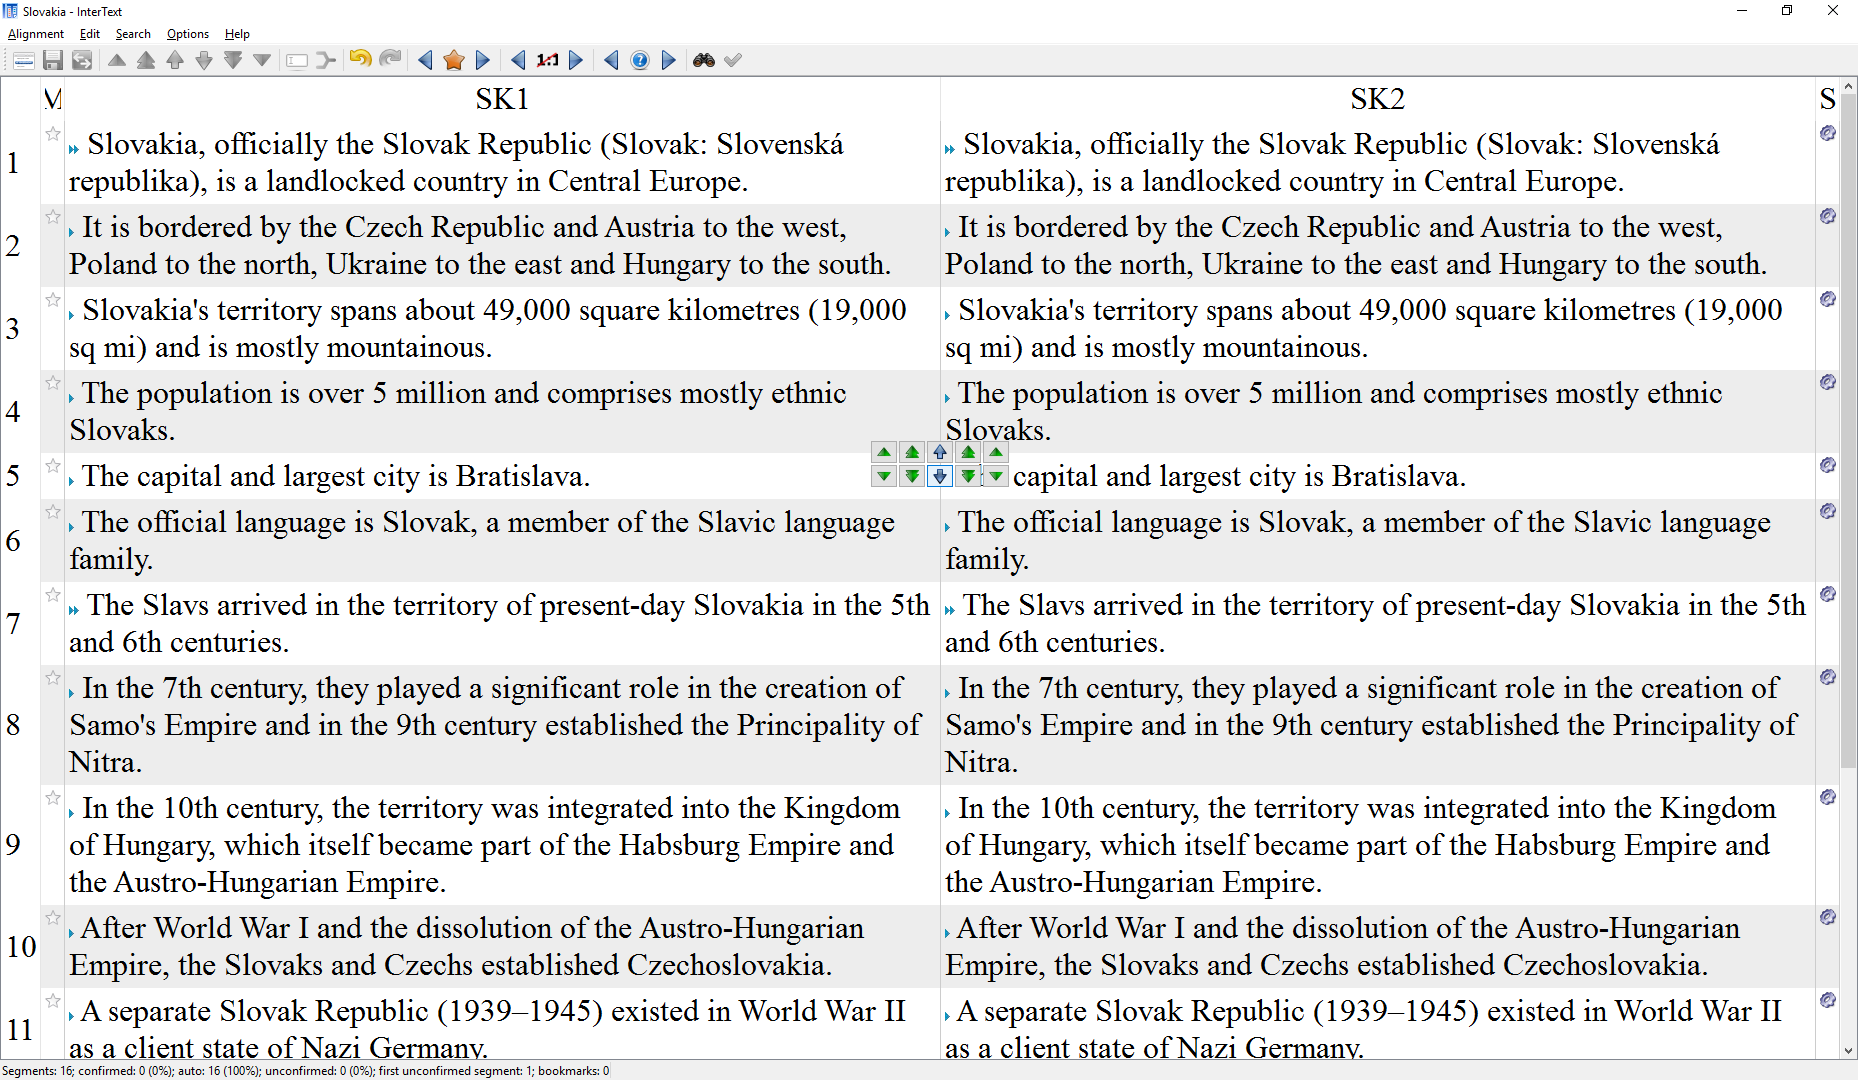
\includegraphics[scale=0.33]{intertext_interface}\end{center}
	\caption[Aplikácia InterText]{Aplikácia InterText}\label{fig:intertext_interface}
\end{figure}

%
% NOVA Text Aligner
%
\ifthenelse {\boolean{bachelor}}
{
	%\subsection{Subsection}
	\subsection{NOVA Text Aligner}
}
{
	%\section{Subsection}
	\section{NOVA Text Aligner}
}
NOVA Text Aligner\footnote{http://www.supernova-soft.com/wpsite/products/text-aligner/} je aplikácia na zarovnávanie textu, pričom nevyužíva algoritmy na zarovnávanie textu, ale používateľ si musí sám určiť zarovnanie.

Ako vidno na obrázku~\fullref{fig:nova_text_aligner_interface} hlavná editovacia časť aplikácie je rozdelené do dvoch častí. Umožňuje do ľavej aj pravej časti načítať rôzny text, v ktorom sa dá veľmi jednoducho vyhľadávať, k čomu napomáha zvýraznenie vyhľadaných slov. Načítaný text je možné premiestňovať a zoskupovať, či už podľa riadkov alebo aj v celých blokoch a nechýba možnosť editovať text. Je možné si túto aplikáciu prispôsobiť. Ponúka možnosti ako zmena typu písma a pod. Finálny spracovaný text sa dá exportovať do viacerých formátov, z ktorých populárne sú formáty elektronických knižiek EPUB a MOBI.

Aplikácia je zameraná hlavne na usporadúvanie textu, nezaznamenáva si používateľove zmeny textu a neprispôsobuje sa podľa toho pri ďalšom použití a funguje iba lokálne. NOVA Text Aligner je dostupná iba v skúšobnej verzií, pre dlhodobé používanie si treba zakúpiť licenciu.

\begin{figure}[H]
	\begin{center}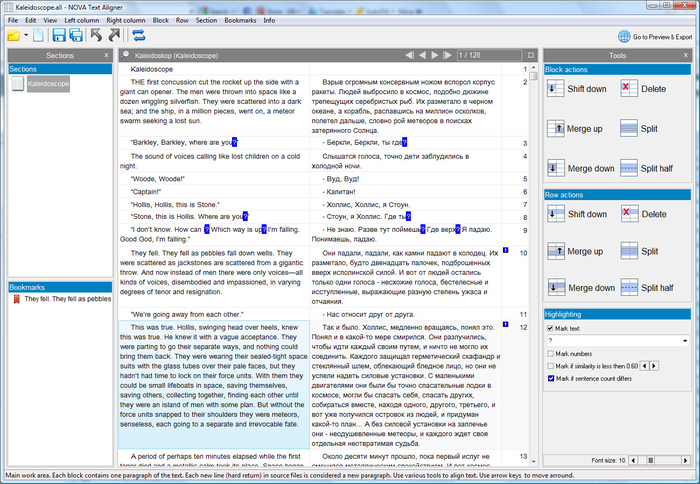
\includegraphics[scale=0.56]{nova_text_aligner_interface}\end{center}
	\caption[Aplikácia NOVA Text Aligner]{Aplikácia NOVA Text Aligner\footnotemark}\label{fig:nova_text_aligner_interface}
\end{figure}
\footnotetext{http://parallel-text-aligner.en.softonic.com/}

%
% LF Aligner
%
\ifthenelse {\boolean{bachelor}}
{
	%\subsection{Subsection}
	\subsection{LF Aligner}
}
{
	%\section{Subsection}
	\section{LF Aligner}
}
Aplikácia LF Aligner\footnote{www.sourceforge.net/projects/aligner} je zameraná na spracovanie textu rôznych jazykov. Ponúka možnosť použiť až 99 jazykov, čo ale znamená 99 vstupných súborov, každý so zvoleným jazykom. Dokáže spracovať rôzne typy vstupných súborov od čistého textu, PDF súborov, cez URL stránok s textom až po správy Európskeho parlamentu, ktoré automaticky stiahne. Výstup môže byť taktiež viacerých druhov, napríklad cez grafické rozhranie LF Aligner alebo vygenerovanie XLS súboru. Na obrázku~\fullref{fig:lf_aligner_interface} vidno grafické rozhranie tejto aplikácie, ktoré ponúka mnohé vymoženosti. Samozrejmosťou je možnosť premiestňovať a zoskupovať riadky, doplnenie ďalšieho súboru na spracovávanie, uloženie zmien súboru prepísaním jeho dát a mnohé ďalšie.

\begin{figure}[H]
	\begin{center}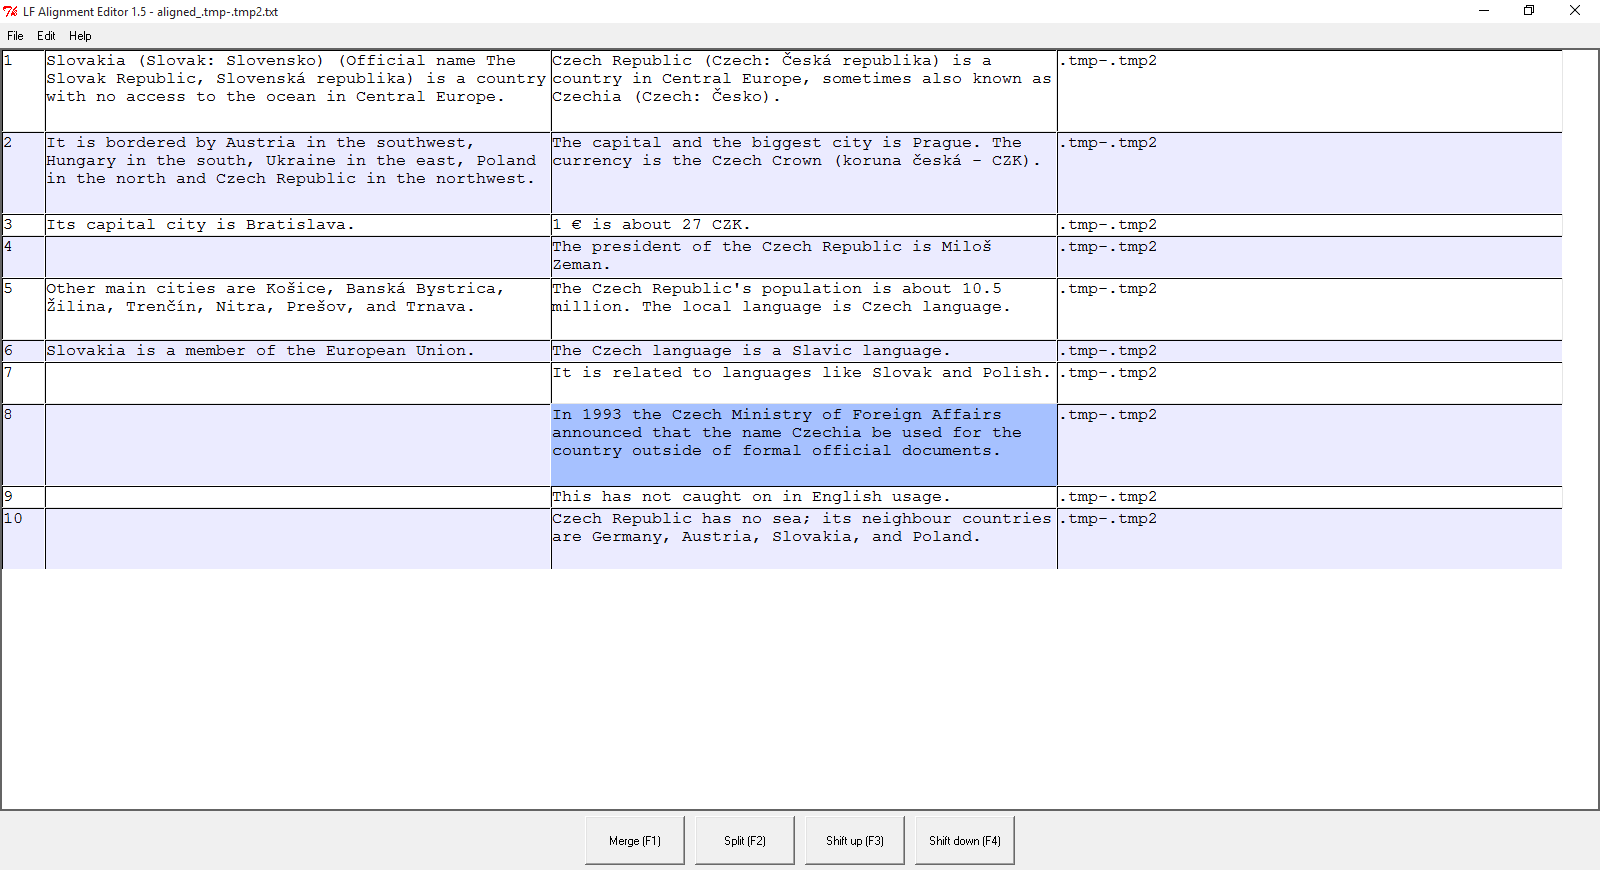
\includegraphics[scale=0.33]{lf_aligner_interface}\end{center}
	\caption[Aplikácia LF Aligner]{Aplikácia LF Aligner}\label{fig:lf_aligner_interface}
\end{figure}
\footnotetext{http://parallel-text-aligner.en.softonic.com/}

%
% Google Translate
%
\ifthenelse {\boolean{bachelor}}
{
	%\subsection{Subsection}
	\subsection{Google Translate}
}
{
	%\section{Subsection}
	\section{Google Translate}
}
Za najznámejšieho zástupcu webových nástrojov na spracovanie paralelných textov sa dá pokladať nástroj Google Translate\footnote{translate.google.com}. Využíva sa na preklad slov, viet, ale dokáže spracovať aj celé texty. Momentálne podporuje preklad z a do 91 jazykov. Dokáže rozpoznať a preložiť hovorenú reč aj písaný text. Pri preklade jednotlivých slov zobrazuje viacero možných prekladov do druhého jazyka, pričom pri preklade z anglického jazyka ponúka aj ukážky viet, v ktorých sa prekladané slovo môže použiť. Správnu výslovnosť preloženého aj prekladaného slova alebo textu, si používateľ môže vypočuť na krátkej zvukovej ukážke.

Na obrázku~\fullref{fig:google_translate_example} je zobrazený preklad anglického textu do slovenského. Vidno, že preklad do minoritných jazykov ešte nie je dokonalý.

\begin{figure}[H]
	\begin{center}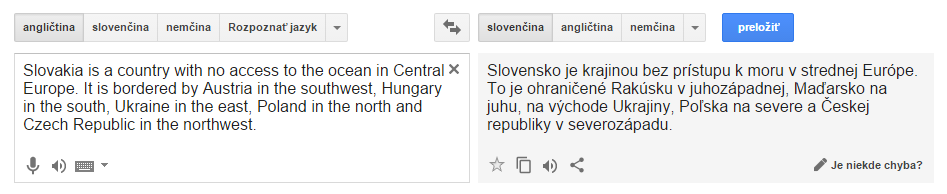
\includegraphics[scale=0.55]{google_translate_example}\end{center}
	\caption[Google Translate]{Google Translate}\label{fig:google_translate_example}
\end{figure}

Analyzované nástroje nespĺňajú všetky požiadavky na systém schopný spoznámkovať učebný text v takom rozsahu, ktorý by umožňoval používateľovi prispôsobiť si spracovaný text. Systém musí umožňovať editáciu jednotlivých viet výstupného textu podľa vôle používateľa. Tieto úpravy musí zohľadniť pri následnej aplikácií transformácií vstupného textu. Dáta ohľadne spoznámkovávania textu musia byť uložené na externom úložisku, ako napríklad v databáze.

%
% Uchovávanie textov v databázach
%
\ifthenelse {\boolean{bachelor}}
{
	%\subsection{Subsection}
	\subsection{Uchovávanie textov v databázach}
}
{
	%\section{Subsection}
	\section{Uchovávanie textov v databázach}
}
\label{subsection:persisting_texts_in_db}
Text je špecifický údajový model s variabilnou štruktúrou. Ak chceme efektívne ukladať texty v databázach, je nutné použiť vhodnú databázu. Databázu, ktorá je tomu prispôsobená, pri ktorej nebudeme zbytočne čerpať pamäť a takisto bude jednoduché narábať s dátami. To znamená bezproblémové ukladanie, získavanie, vyhľadávanie a spracovanie textov na úrovni databázy. V nasledujúcich kapitolách sa pozrieme, aké typy databáz existujú a aké možnosti z pohľadu ukladania textov ponúkajú.

%
% Relačné databázy
%
\ifthenelse {\boolean{bachelor}}
{
	%\subsection{Subsection}
	\subsubsection{Relačné databázy}
}
{
	%\section{Subsection}
	\subsection{Relačné databázy}
}
\label{subsubsection:relation_dbs}
Relačné databázy boli dlhé roky populárnou a finančne nenáročnou voľbou pri tvorbe veľkých podnikateľských aplikácií. Momentálne sú používané vo väčšine súčasných aplikácií a pracujú spoľahlivo pri obmedzenom množstve dát~\cite{MongoDBvsMySQL2015}. Problém s relačným modelom relačných databáz nastáva, keď vzniká potreba aplikácie s obrovským množstvom dát. Menovite rozšíriteľnosť (angl. scalability) a schéme sa stávajú najväčším problémom relačných databáz~\cite{NoSQLDBvsRealtionDB}.

Tento typ databáz oplýva veľkou úrovňou jednotvárnosti, ukladá dáta v tabuľkách zložených z riadov a stĺpcov. Každý záznam (riadok) v tabuľke predstavuje zjednodušený objekt alebo vzťah z reálneho života. Výhodou relačných databáz je možnosť jednoduchého vytvorenia prispôsobeného pohľadu na dáta~\cite{Maier}.

%
% Textové databázy
%
\ifthenelse {\boolean{bachelor}}
{
	%\subsection{Subsection}
	\subsubsection{Textové databázy}
}
{
	%\section{Subsection}
	\subsection{Textové databázy}
}
\label{subsubsection:text_dbs}
S rozmachom variácie dát v posledných rokoch sa začali objavovať a vznikať nerelačné databázy, aby pokryli požiadavky na nové aplikácie. Textové databázy sú druhom nerelačných databáz.

Textové databázy ukladajú dáta vo forme dokumentov, vďaka čomu ponúkajú vysoký výkon a horizontálnu rozšíriteľnosť~\cite{NoSQLDBvsRealtionDB}. Uložené dokumenty môžu nadobúdať rôzne formáty, ako napríklad JSON, BSON, XML a BLOB, ktoré poskytujú veľkú flexibilnosť pre dáta. Každý záznam v takejto databáze preto môže mať inú štruktúru, napríklad počet alebo typ polí, čo šetrí úložným priestorom, keďže neobsahuje nepotrebné prázdne polia~\cite{NoSQLDBvsRealtionDB}.

Dokumenty v databáze sú referencované kľúčom, ktorý môže byť reťazec, cesta, ale dokonca aj dokument~\cite{NoSQLDBvsRealtionDB}. Majú dynamickú schému, čo umožňuje vytvárať záznamy bez toho, aby bolo potrebné predtým definovať štruktúru. Uľahčujú zmenu štruktúry záznamov jednoduchým pridaním, odstránením alebo zmenou typu poľa. Vďaka svojej štruktúre sú dokumenty ľahko namapovateľné na objekty z objektovo-orientovaných programovacích jazykov a odstraňujú tým potrebu pre použitie objektovo-relačnej mapovacej vrstvy.
\\

Primárne využitie týchto databáz je v aplikáciách, ktoré potrebujú ukladať dáta, ktorých štruktúra je vopred neznáma alebo sa mení. Predstaviteľmi sú napríklad \textit{MongoDB} alebo \textit{CouchDB} databázy.

%
% MongoDB
%
\ifthenelse {\boolean{bachelor}}
{
	%\subsection{Subsection}
	\paragraph{MongoDB}
}
{
	\%section{Subsection}
	\subsubsection{MongoDB}
}
\label{subsection:mongodb}
MongoDB\footnote{www.mongodb.org} je dokumentová nerelačná databáza vytvorená v C++ spustená v roku 2009~\cite{NoSQLDBvsRealtionDB}. Ukladá dáta v dokumentoch vo formáte BSON (Binary JSON), ktorých štruktúra sa môže meniť. Využíva dynamickú štruktúru schém, preto dokáže vytvárať záznamy bez preddefinovanej štruktúry dát, lebo štruktúra sa vytvára za behu, pričom môže byť veľmi jednoducho pozmenená pridaním, odstránením alebo zmenou typu polia dokumentu určujúceho štruktúru. Umožňuje jednoduché ukladanie dát s hierarchickými vzťahmi alebo komplexnejších štruktúr, ako sú napríklad polia, listy alebo vnorené polia.

Vlastnosti ako chybová tolerancia, perzistencia a konzistencia dát sú súčasťou MongoDB. Oproti klasickým dokumentovým databázam ponúka aj vymoženosti, ako agregácia, ad hoc dopyty, indexovanie, a pod. Taktiež má svoj vlastný plnohodnotný dopytovací jazyk \textit{mongo query language}~\cite{NoSQLDBvsRealtionDB}.

Prvky poskytované databázou MongoDB sú prvky zahrnuté v relačných databázach rozšírené o ďalšiu funkcionalitu. Porovnanie poskytovaných prvkov je v tabuľke~\fullref{table:features_of_mongodb}. 

\begin{table}[H]
	\centering
	\caption{Prvky poskytované MongoDB}
	\label{table:features_of_mongodb}
	\begin{tabular}{|l|l|l|}
		\hline
		& \textbf{MySQL} & \textbf{MongoDB} \\ \hline
		Bohatý dátový model & Nie & Áno \\ \hline
		Dynamická štruktúra & Nie & Áno \\ \hline
		Dátové typy & Áno & Áno \\ \hline
		Lokálnosť dát & Nie & Áno \\ \hline
		Aktualizovanie polí & Áno & Áno \\ \hline
		Ľahké pre programátorov & Nie & Áno \\ \hline
		Komplexné transakcie & Áno & Nie \\ \hline
		Audit & Áno & Áno \\ \hline
		Auto-sharding & Nie & Áno \\ \hline
	\end{tabular}
\end{table}

Bohatý dátový model (angl. Rich Data Model) znamená, že dátový model poskytuje veľa funkcionality. Princípom dynamickej štruktúry (angl. Dynamic Structure) je jednoduchá zmena štruktúru, pričom nemusí byť vôbec zadefinovaná a každý záznam môže mať odlišnú štruktúru. Lokálnosť dát (angl. Data Locality) znamená uchovávanie súvisiacich dát pokope. Aktualizovanie polí umožňuje vykonávať nad poliami operácie, ako sú inkrementácia podľa špecifikovaného množstva, vynásobenie hodnotou, premenovanie, aktualizácia iba ak je hodnota väčšia alebo menšia ako špecifická hodnota a ďalšie. Audit (angl. Auditing) je funkcionalita, ktorá umožňuje administrátorom a používateľom sledovať aktivity systému.
Auto-sharding pri náraste dát, aby sa zabránilo poklesu priepustnosti operácií čítania a zapisovania, ukladá dáta automaticky na viacero strojov.

MongoDB má vlastnú konvenciu názvov svojich častí. Tie sa v niektorých prípadoch líšia s názvami relačných databáz. Rozdiely sú zobrazene v tabuľke~\fullref{table:names_of_mongodb}. Za zástupcu relačných databáz bola vybraná MySQL databáza. 

\begin{table}[H]
	\centering
	\caption{Porovnanie používaných pojmov~\cite{MongoDBvsMySQL2015}}
	\label{table:names_of_mongodb}
	\begin{tabular}{|l|l|}
		\hline
		\textbf{MySQL} & \textbf{MongoDB} \\ \hline
		Databáza & Databáza \\ \hline
		Tabuľka & Kolekcia \\ \hline
		Index & Index \\ \hline
		Riadok & BSON dokument \\ \hline
		Stĺpec & BSON pole (angl. field) \\ \hline
		Spojenie & Vnorené dokumenty a prepojenie \\ \hline
		Primárny kľúč & Primárny kľúč \\ \hline
		Zoskupenie & Agregácia \\ \hline
	\end{tabular}
\end{table}

%
% Ostatné databázové systémy
%
\ifthenelse {\boolean{bachelor}}
{
	%\subsection{Subsection}
	\subsubsection{Ostatné databázové systémy}
}
{
	\%section{Subsection}
	\subsection{Ostatné databázové systémy}
}
\label{subsection:types_of_norelation_dbs}
Okrem relačných a textových dokumentov existuje ešte niekoľko druhov databáz. V nasledujúcich častiach si priblížime niektoré z nerelačných databáz.

%
% Kľúč - hodnota databázy
%
\ifthenelse {\boolean{bachelor}}
{
	%\subsection{Subsection}
	\paragraph{Kľúč - hodnota databázy}
}
{
	\%section{Subsection}
	\subsubsection{Kľúč - hodnota databázy}
}
\label{subsubsection:key_value_db}
Nerelačné databázy typu kľúč - hodnota sú v svojej podstate celkom jednoduché, ale zároveň efektívne. Umožňujú používateľovi ukladať dáta ľubovoľne, kedže neobsahujú schémy. Uložené dáta sa skladajú z dvoch častí. Prvá časť je kľuč a druhá časť je hodnota~\cite{NoSQLDBvsRealtionDB}, pričom kľúč je samo-generujúci string a hodnota môže byť takmer čokoľvek, od string, JSON cez BLOB až po obrázok~\cite{MongoDBvsMySQL2015}.

Kľúč - hodnota databázy sú veľmi podobné hašovacím tabuľkám, kde kľúč je indexom do tabuľky, pomocou ktorého používateľ môže pristúpiť k hodnote daného kľúču. Tento typ databáz uprednostňuje rozšíriteľnosť pred konzistenciou. Ponúka vysokú konkurenčnosť (angl. concurrency), rýchle vyhľadávanie a schopnosť uloženia veľkého množstva dát za cenu spojovacích a agregačných operácií. Taktiež je veľmi náročné vytvoriť ľubovoľný pohľad na dáta z dôvodu chýbajúcej schémy~\cite{NoSQLDBvsRealtionDB}.

Najznámejšími predstaviteľmi tohto typu databáz sú \textit{Amazon DynamoDB} a \textit{RIAK}.

%
% Stĺpcové databázy
%
\ifthenelse {\boolean{bachelor}}
{
	%\subsection{Subsection}
	\paragraph{Stĺpcové databázy}
}
{
	\%section{Subsection}
	\subsubsection{Stĺpcové databázy}
}
\label{subsubsection:column_db}
Stĺpcové databázy musia mať preddefinovanú schému, v ktorej sú jednotlivé bunky záznamov zoskupené do kolekcie stĺpcov~\cite{MongoDBvsMySQL2015}. Dáta nie sú ukladané do tabuliek, ale do masívne distribuovaných architektúr, s hlavným zámerom, aby agregácia dát mohla prebehnúť veľmi rýchlo s redukovaním I/O aktivity.

Tento typ databáz taktiež poskytuje veľkú rozšíriteľnosť v ukladaní dát.

Najvhodnejšie je využívať stĺpcové databázy v analytických aplikáciách alebo aplikáciách, ktoré získavajú dáta pomocou metódy \textit{data mining}~\cite{NoSQLDBvsRealtionDB}.

%
% Grafové databázy
%
\ifthenelse {\boolean{bachelor}}
{
	%\subsection{Subsection}
	\paragraph{Grafové databázy}
}
{
	\%section{Subsection}
	\subsubsection{grafové databázy}
}
\label{subsubsection:graph_db}
Grafové databázy su špeciálny typ databáz, v ktorých sú dáta uložené vo forme grafu. Graf pozostáva z vrcholov a hrán, pričom vrcholy predstavujú objekty a hrany reprezentujú vzťahy medzi nimi. Každý vrchol okrem iného obsahuje aj ukazovateľ na priľahlé vrcholy, čo umožňuje prechádzať obrovské množstvo dát rýchlejšie ako v relačných databázach~\cite{NoSQLDBvsRealtionDB}.

Údaje sa ukladajú v polo-štruktúrovanej forme, kde je kladený hlavný dôraz na prepojenia medzi dátami. Grafové databázy spĺňajú vlastnosť ACID a sú veľmi vhodné pre biometrické aplikácie alebo aplikácie sociálnych sietí. Hlavným predstaviteľom grafových databáz je \textit{Neo4j}~\cite{NoSQLDBvsRealtionDB}.

%
% Objektovo orientované databázy
%
\ifthenelse {\boolean{bachelor}}
{
	%\subsection{Subsection}
	\paragraph{Objektovo orientované databázy}
}
{
	\%section{Subsection}
	\subsubsection{Objektovo orientované databázy databázy}
}
\label{subsubsection:object_oriented_db}
Objektovo orientované databázy ukladajú dáta vo forme objektov, rovnako ako sú údaje reprezentované v objektoch v objektovo orientovaných programovacích jazykoch (OOP). Tieto databázy podporujú všetky vymoženosti OOP, ako enkapsulácia, polymorfizmus, ale aj dedenie. Objektovo orientované databázy robia moderný vývoj softvéru jednoduchším~\cite{NoSQLDBvsRealtionDB}.

%
% Zhrnutie aplikácií na spracovanie prirodzeného jazyka
%
\ifthenelse {\boolean{bachelor}}
{
	%\subsection{Subsection}
	\subsection{Zhrnutie}
}
{
	%\section{Subsection}
	\section{Zhrnutie}
}
\label{subsection:analysis2:zhrnutie}
Analyzovali sme aplikácie, ktoré umožňujú spravovať a editovať paralelný text. Za ich pomoci dokážeme zo vstupného textu získať výstupný text. Napríklad pri preklade máme vstupný text množinu viet v anglickom jazyku, ktorú chceme preložiť do slovenského jazyka a výstupný text je preloženú množinu viet. Pri zjednodušovaní textu je na vstupe taktiež množina viet a na výstupe je každá veta zo vstupnej množiny zjednodušená podľa istých pravidiel. Výstupný text vzniká určitou transformáciou vstupného textu, aplikovaním transformácie na každú vetu zdrojového textu.\\

[TREBA TO TU NEJAK PREPOJIT, KEDZE TEXT HORE JE ZO ZHRNUTIA NASTROJOV A TEXT POD JE ZO ZHRNUTIA DATABAZ - SPOJIT DO JEDNEHO ZHRNUTIA CELEJ KAPITOLY !!!]\\

NOSQL databáza je narozdiel do RDBMS modelu (Relation Data Base Management System)
navrhnutá, tak aby bola jednoducho rozšíriteľná so zväčšovaním dát. Väčšina NOSQL databáz odstránila niektoré nepotrebné prvky RDBMS modelov, čím sa stali podstatne ľahšími a efektívnejšími. Toto na druhej strane spôsobilo, že NOSQL model negarantuje vlastnosti ACID (Atomicity, Consistency, Isolation, Durability), ale naopak garantuje vlastnosti BASE (Basically Available, Soft state, Eventula Consistency)~\cite{NoSQLDBvsRealtionDB}.

Nerelačné databázy neukladajú údaje v tabuľkách a nemajú fixnú schému. Tieto vlastnosti im umožňujú jednoducho spracovávať neštruktúrované dáta, ako sú dokumenty, e-maily a mnoho ďalších~\cite{MongoDBvsMySQL2015}. Preto majú čím ďalej, tým viac využití.

Existuje hneď niekoľko prípadov, kedy je lepšie použiť nerelačnú databázu namiesto relačnej databázy. Keď je potrebné, aby aplikácia dokázala spracovávať rôzne typy a tvary dát alebo pri potrebe spravovať aplikáciu efektívnejšie pri rozširovaní, je rozhodne výhodnejšie použiť nerelačnú databázu. Niektoré databázy, ako napríklad textová databáza MongoDB uľahčuje vývoj aplikácií, keďže jeho dokumentová štruktúra dát je jednoducho namapovateľná na moderné, objektovo-orientované programovacie jazyky a tým pádom nie je potreba využívať komplexnú objektovo-relačnú mapovaciu vrstvu, ktorá je nutná pri použití relačných databáz na prevod objektov z programovacie jazyka na perzistentné objekty v databáze. Všeobecne je omnoho ľahšie rozšíriť schému / model nerelačnej databázy ako rozširovať schému relačnej databázy.

V systéme potrebujeme ukladať v databáze texty a informácie o nich. Počet viet, slov, vzťahov je pre každý text odlišný a preto nedokážeme vopred definovať efektívnu schému na ukladanie týchto dát. Textové databázy, so svojou dynamickou a ľahko upraviteľnou štruktúrou, sú na tento účel ideálne, pričom ukladanie textov v tabuľkách by bolo náročne, navyše relačné databázy nemajú predvolené podporované vyhľadávania v štruktúrach ako text. MongoDB (viď.~\fullref{subsection:mongodb}) je vyspelá, dokumentová databáza zahrňajúca všetku funkcionalitu, ktorú potrebujeme.